\section{\label{sec:selection}Event selection}
The event selection described in \cite{duet} used the PIA$\nu$O detector to identify events with no $\pi^{+}$ in the final state which are consistent with ABS+CX final states. As mentioned, for the analysis presented in this paper the selection was extended by using information from the downstream detector CEMBALOS to identify photons following a CX interaction. 

An illustration of a simulated CX event is shown in Fig. \ref{fig:event}. The upstream horizontal (red) track represents a $\pi^{+}$ interacting in the PIA$\nu$O detector. As it undergoes a CX interaction two protons (black) and a $\pi^{0}$ are produced. The $\pi^{0}$ subsequently decays into two photons (blue). The forward-going photon travels to CEMBALOS where it converts into $e^{+}$-$e^{-}$ pairs and deposits charge in the scintillating material.

\begin{figure}[ht]
%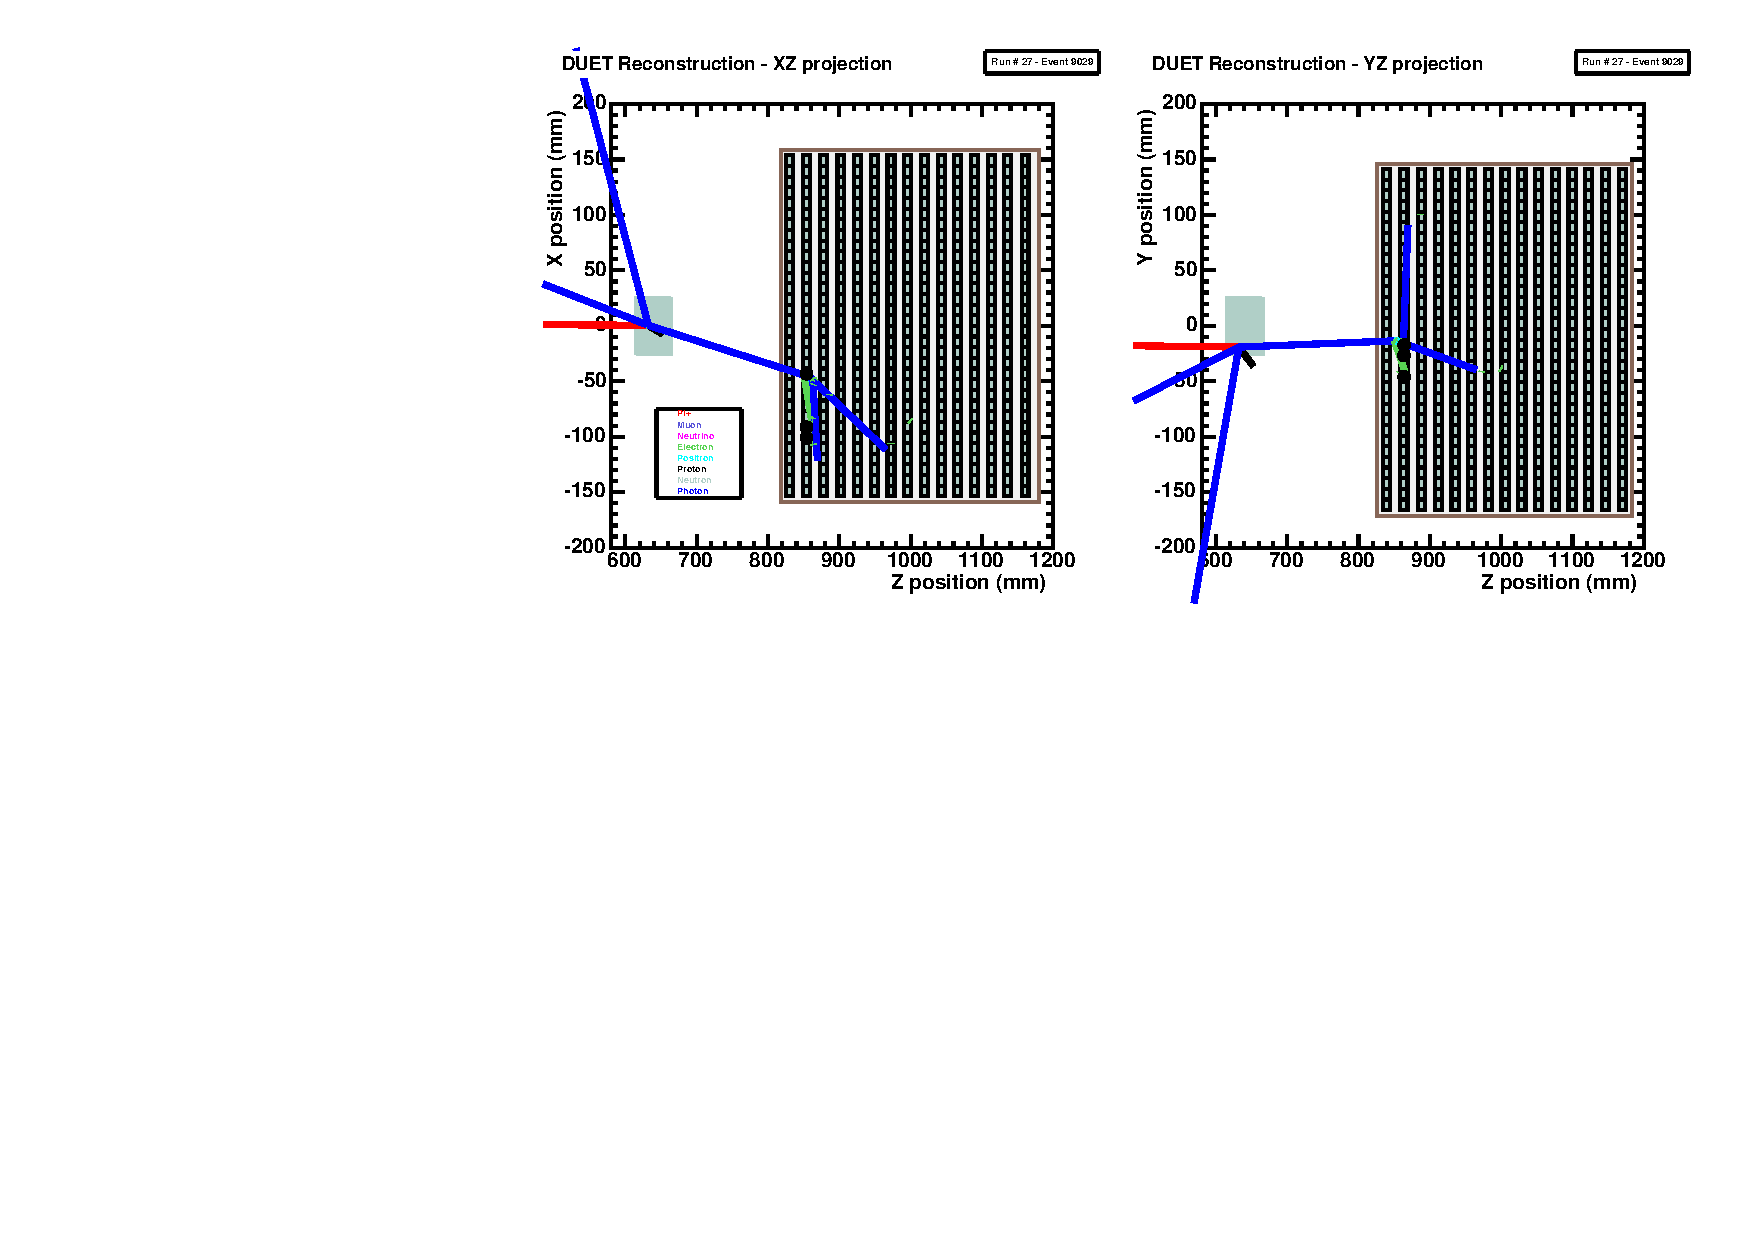
\includegraphics[width=90mm]{figures/ev_display_27_9029_intr4_ntag267.pdf}
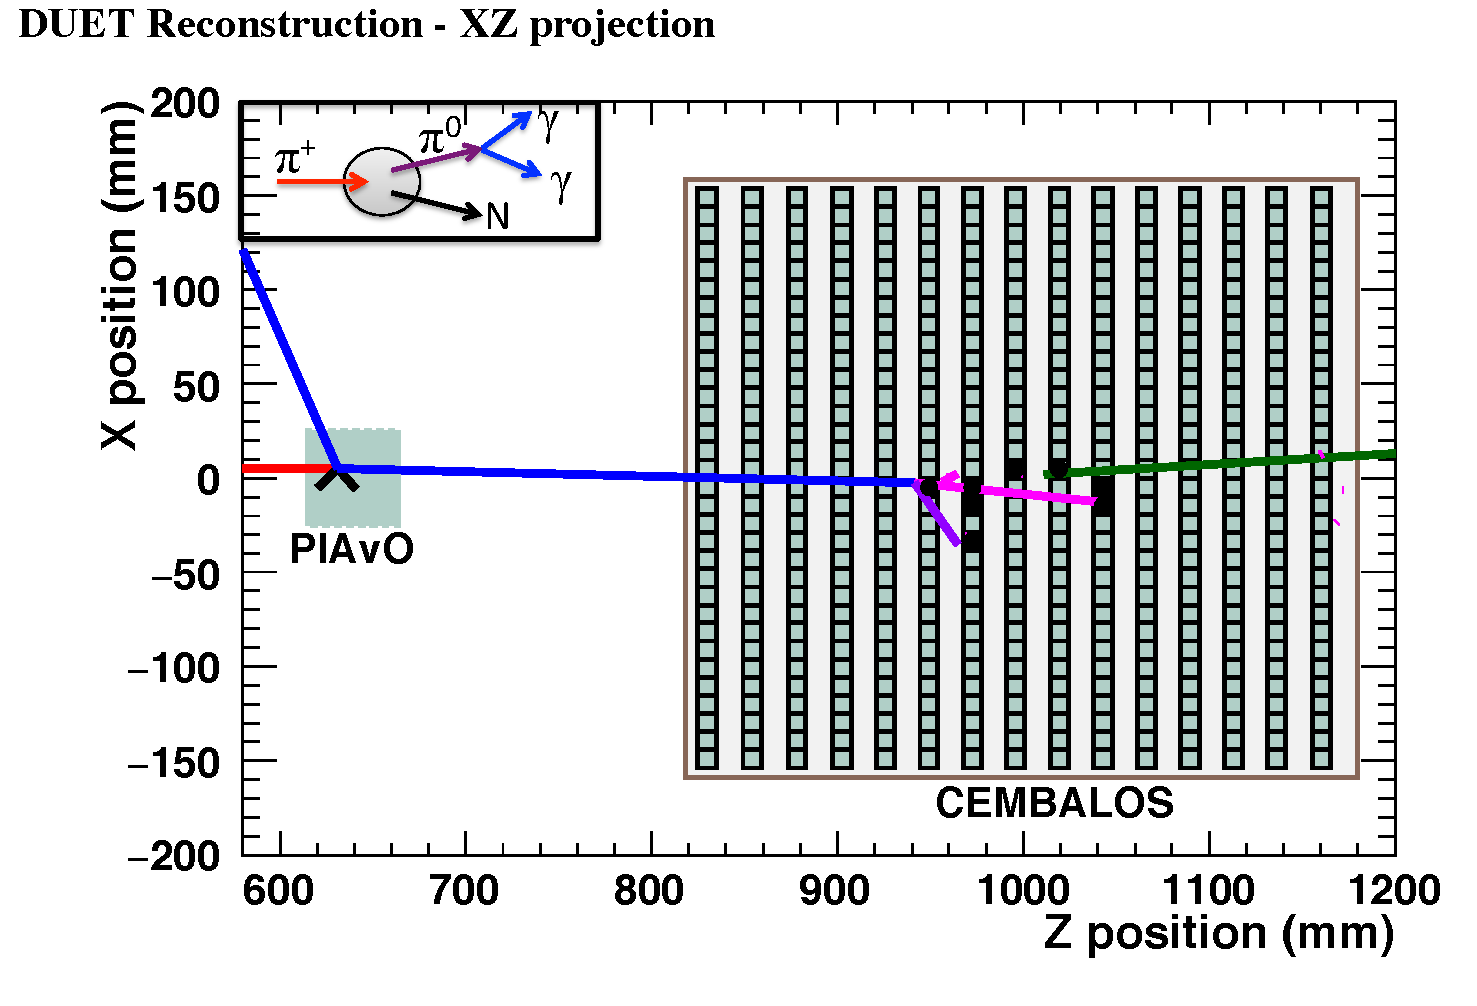
\includegraphics[width=90mm]{figures/event_display_with_diagram.pdf}
\caption{(Color online) Example of a simulated CX event in the DUET detector setup. A 237.2 MeV$/c$ $\pi^+$ (red) undergoes CX in PIA$\nu$O producing two protons (black) and a $\pi^0$ that decay into two photons (blue). The forward-going photon is identified in CEMBALOS as it produces $e^{+}$-$e^{-}$ pairs (purple, magenta) and hits are recorded in the scintillating material.}
\label{fig:event}
\end{figure}

\subsection{PIA$\nu$O upstream selection}
The PIA$\nu$O detector track reconstruction algorithm used charge deposition information to reconstruct and identify charged particles in the detector and to identify an interaction vertex within a defined fiducial volume (FV). A detailed description can be found in Sec. III of \cite{duet}. A summary of the upstream selection criteria follows:
\begin{enumerate}
\item {\bf Good incident $\pi^{+}$\\}
This selection criteria is threefold: firstly, an incident $\pi^{+}$ was selected using TOF and Cherenkov light information. Secondly, a straight track, normal to the incident plane, leaving hits in the first 5 layers was required. Thirdly, this incident track was required to enter a defined fiducial volume (FV).
\item {\bf Vertex inside the FV\\}
Events with pion interactions were selected by requiring a reconstructed vertex inside the FV. This removed through-going and pion events, as well as small-angle scattering events.
\item {\bf No $\pi^{+}$ final track\\}
Reconstructed tracks exiting the interaction vertex were classified into ``proton-like" and ``pion-like" tracks using an angle-dependent cut on the deposited charge, $dQ/dx$. Events with no ``pion-like'' tracks in the final state were selected.
\end{enumerate}
There were $\sim$7000 selected events in data after these criteria were applied with a $\sim$79\% efficiency to select ABS+CX events occurring inside the FV. The purity was estimated to be $\sim$73\%. The main backgrounds were $\pi^{+}$ elastic and quasi-elastic scatterings. This selection was used to extract $\sigma{_\mathrm{ABS+CX}}$ in \cite{duet}.

\subsection{CEMBALOS selection}
Charge deposition information from CEMABALOS was used to identify CX interactions occurring in PIA$\nu$O. The main goal was to tag one of the photons from the decay of a $\pi^0$ by identifying the corresponding electromagnetic shower in CEMBALOS. The limited angular coverage ($\sim0.53 sr$) of CEMBALOS imposed the largest efficiency loss. The selection criteria were as follows:
\begin{enumerate}
\item{\bf Veto cut\\}
Charged particles in CEMBALOS left a signal in the scintillator material. Fig. \ref{fig:veto} shows the distribution of the position of the most upstream hit in CEMBALOS for each event. Each bar represents a scintillation plane. A veto cut on the first two layers was applied to remove most of the charged particle backgrounds, such as as low-angle $\pi^+$ scatters and protons from ABS events.

\begin{figure}[ht]
 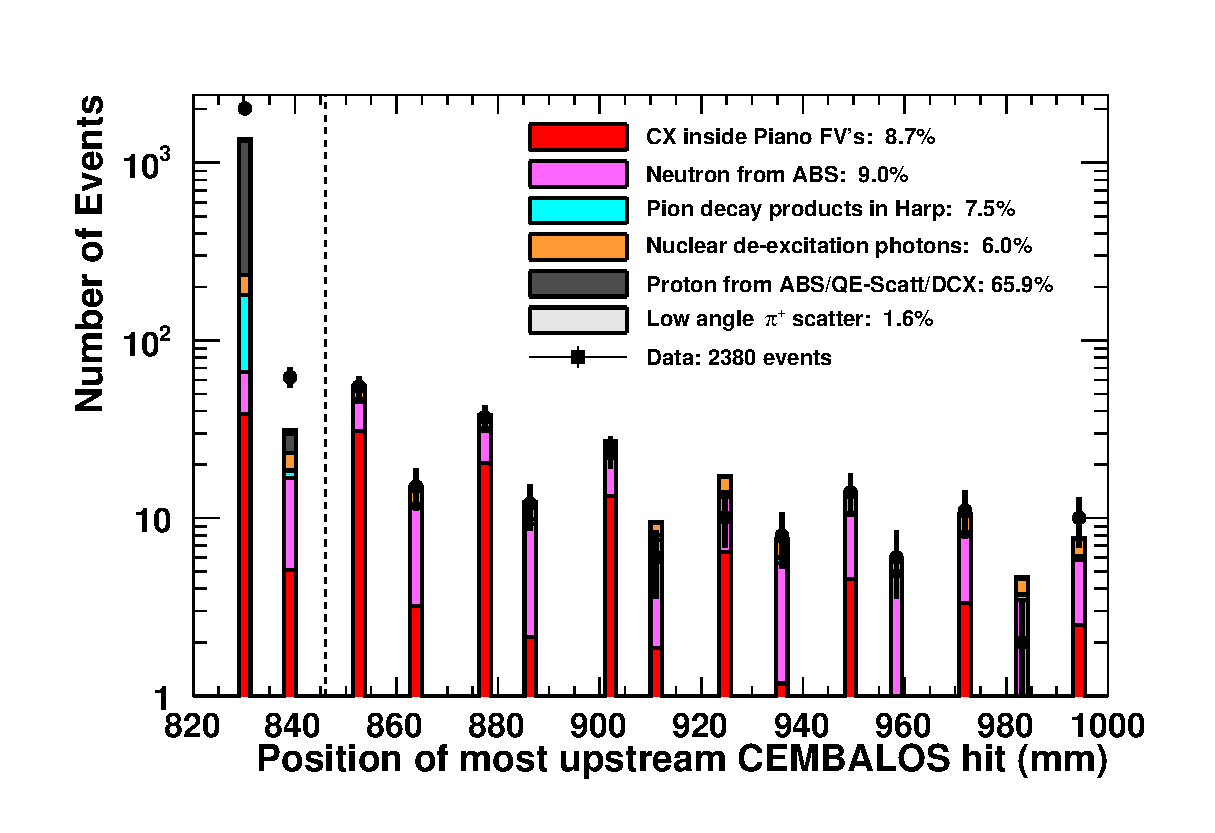
\includegraphics[width=86mm]{figures/duettag_fgdMostUp_10000_forpaper_v2.eps}
 \caption{(Color online) Distribution of the most upstream position of CEMABLOS hits for Data and MC in the $p_\pi=$237.2 MeV$/c$ setting after applying the PIA$\nu$O upstream selection. Each bar represents an XY module. Topologies contributing less than 1\% are not plotted.}
 \label{fig:veto}
\end{figure}
   
\item{\bf Hit Charge vs. Multiplicity\\}
Neutrons from ABS events and nuclear de-excitation $\gamma$-rays mostly produced hits after the first two modules. Fig. \ref{fig:nhits} shows the distribution of the number of hits (multiplicity) in CEMBALOS. A minimum of five hits was required to reduced these background sources. Fig. \ref{fig:nhitsvsCharge} shows the CEMBALOS hit charge vs. multiplicity distribution after applying the veto cut. A diagonal cut in this plane was applied to further reduce the remaining background of neutrons from ABS.
\end{enumerate}

\begin{figure}[ht]
 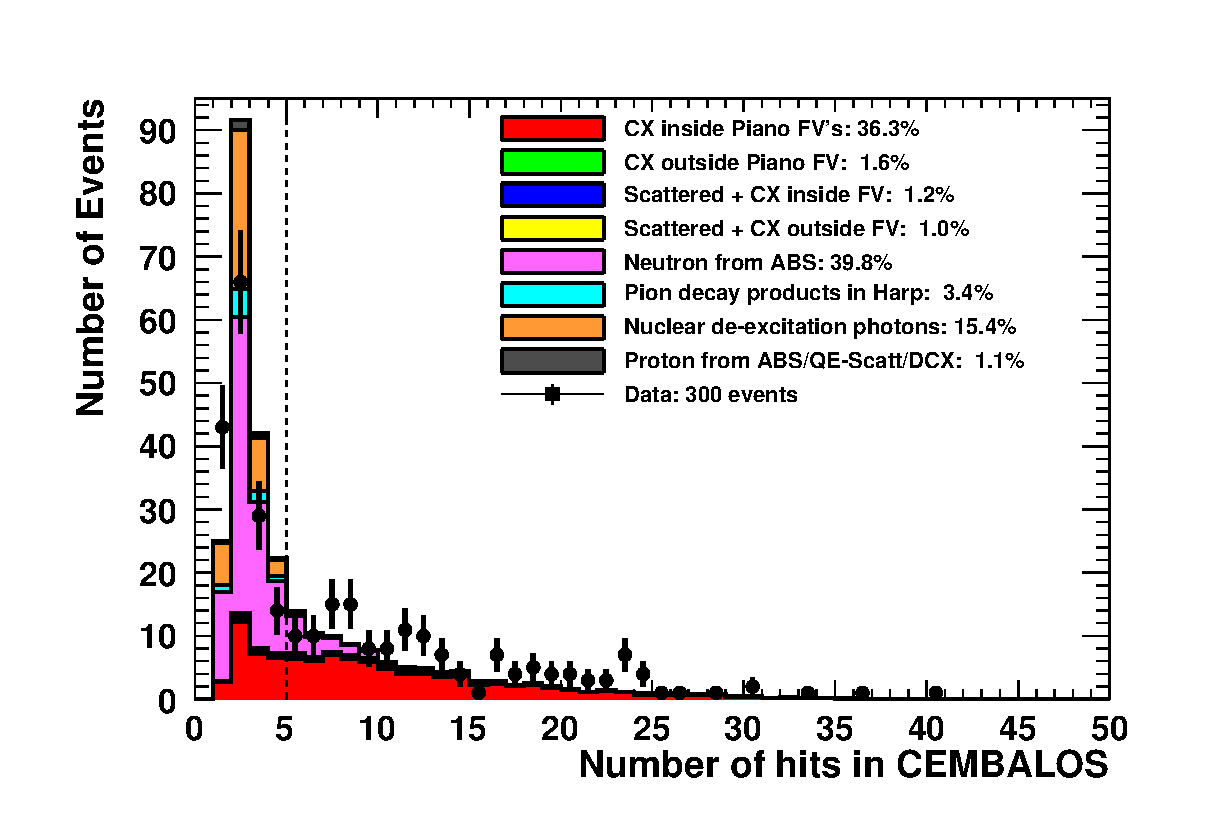
\includegraphics[width=86mm]{figures/duettag_nhits_20000_forpaper_v2.eps}
 \caption{(Color online) Distribution of the number of hits in CEMABLOS for Data and MC in the $p_\pi=$237.2 MeV$/c$ setting after applying the veto cut.}
 \label{fig:nhits}
\end{figure}

\begin{figure}[ht]
 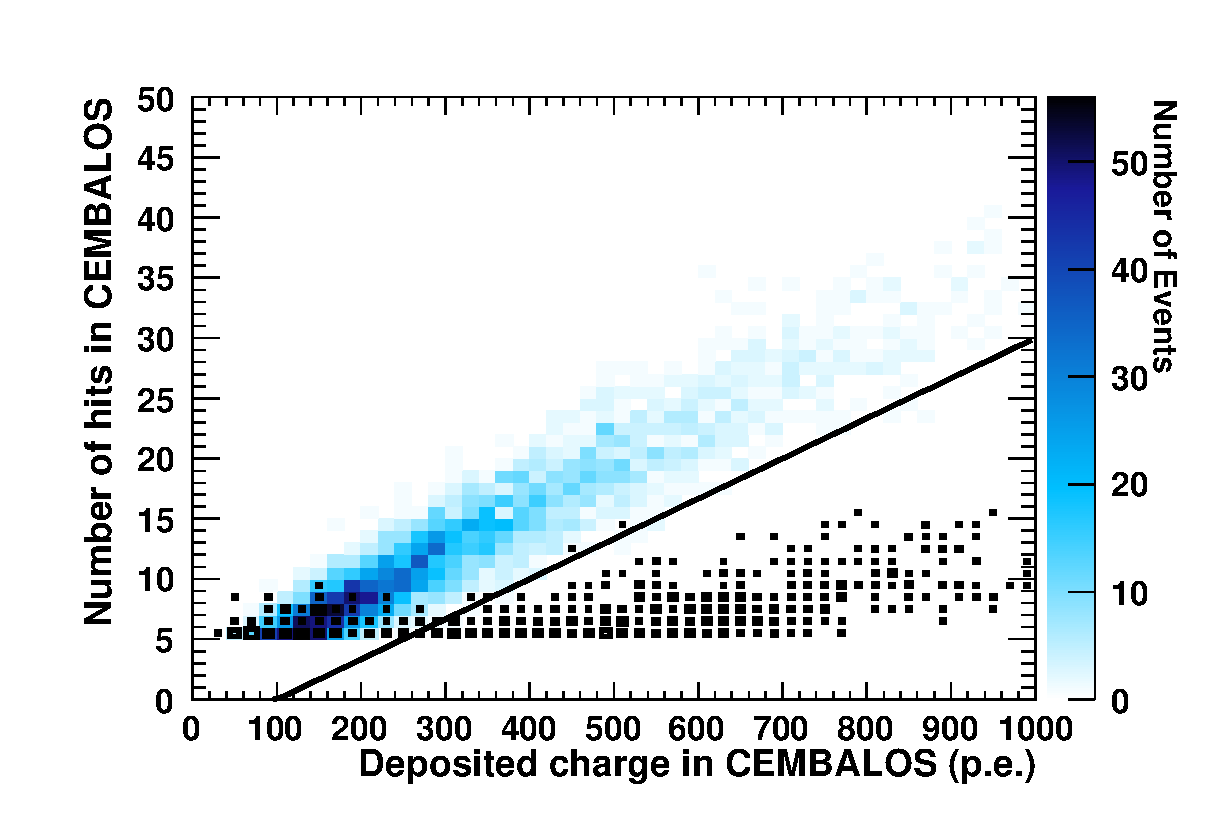
\includegraphics[width=86mm]{figures/draw2Dcut_draw.eps}
 \caption{(Color online) Distribution of the number of hits in CEMABLOS vs. charge deposited for Data and MC in the $p_\pi=$237.2 MeV$/c$ setting after applying the requirement of a minimum of 5 hits. The blue entries are true CX events, whereas the black boxes correspond to neutron background events.}
 \label{fig:nhitsvsCharge}
\end{figure}


\subsection{Selection purities and efficiencies}
The numbers of selected events for each momentum setting after the PIA$\nu$O and CEMBALOS selections were applied are summarized in Table \ref{tbl:short_event_summary} for data $N_{\mathrm{Data}}$ and MC (split into signal $N_{\mathrm{CX}}^{\mathrm{MC}}$ and background $N_{\mathrm{BG}}^{\mathrm{MC}})$. There are $\sim$100 events in data after the event selection, except for the 216.6 MeV$/c$ setting. The efficiencies and purities to select CX events which occurred inside the fiducial volume were around $\sim6\%$ and $\sim90\%$ respectively.

\begin{table}[h]
   \begin{tabular}{c|ccccc}
    \noalign{\hrule height 1pt}
    $p_{\pi}$  [MeV$/c$] & $N_{\mathrm{Data}}$ & $N_{\mathrm{CX}}^{\mathrm{MC}}$ & $N_{\mathrm{BG}}^{\mathrm{MC}}$ & Efficiency [\%] & Purity [\%] \\\hline
    201.6 & 104 & 60.4 & 8.6 & 5.1 & 87.5  \\
    216.6 & 20  & 15.8 & 2.4 & 5.3 & 86.6  \\
    237.2 & 141 & 75.9 & 11.1 & 5.9 & 87.2  \\
    265.6 & 152 & 87.1 & 10.4 & 7.0 & 89.3  \\
    295.1 & 163 & 119.4 & 12.8 & 8.1 & 90.3  \\
    \noalign{\hrule height 1pt}
   \end{tabular}
\caption{Summary of number of events selected after the CEMBALOS downstream selection in Data and MC for each momentum setting, along with estimated efficiencies and purities.}
\label{tbl:short_event_summary}
\end{table}

\section{$\sigma_{\mathrm{CX}}$ and $\sigma_{\mathrm{ABS}}$ extraction}\label{sec:xsec}
After the event selection described above, $\sigma_{\mathrm{CX}}$ is obtained as in \cite{duet} for $\sigma_{\mathrm{ABS+CX}}$. Corrections for the fraction of muons in the beam ($f_{\mu}$) and the fraction of interactions on TiO$_2$ nuclei ($R_{\mathrm{TiO}_2}^{\mathrm{Data}}$ and $R_{\mathrm{TiO}_2}^{\mathrm{MC}}$) were applied as shown in (\ref{eqn:xsec_calc}).

 \begin{equation} \label{eqn:xsec_calc}
 \begin{aligned}
 \sigma_{\mathrm{CX}} &= 
 \sigma_{\mathrm{CX}}^{\mathrm{MC}}
 \times \frac{N_{\mathrm{Data}}-N_{\mathrm{BG}}^{\mathrm{MC}}}{N_{\mathrm{CX}}^{\mathrm{MC}}} \\
 &\times
 \frac{1-R_{\mathrm{TiO}_2}^{\mathrm{Data}}}{1-R_{\mathrm{TiO}_2}^{\mathrm{MC}}}
 \times \frac{1}{1-f_{\mu}},
 \end{aligned}
 \end{equation} 
 
where $\sigma_{\mathrm{CX}}^{\mathrm{MC}}$ is the CX cross section predicted by the simulation. $\sigma_{\mathrm{ABS}}$ is obtained by subtracting $\sigma_{\mathrm{CX}}$ from $\sigma_{\mathrm{ABS+CX}}$ from \cite{duet}.
 